% ----------------------------------------------------------------
% AMS-LaTeX Paper ************************************************
% **** -----------------------------------------------------------
\documentclass[oneside]{amsart}
\usepackage{graphicx}
\usepackage{color}
\usepackage[letterpaper]{geometry}
\usepackage[colorlinks=false,
            pdfborder={0 0 0},
            pdftitle={CSC469 A1},
            pdfauthor={Daniel Bloemendal},
            pdfsubject={CSC469},
            pdfstartview=FitH,
            pdfmenubar=false,
            pdfdisplaydoctitle=true,
            bookmarks=false]{hyperref}
\usepackage{caption}
\usepackage{subcaption}
\usepackage{mathtools}
\usepackage{epstopdf}
% ----------------------------------------------------------------
\vfuzz2pt % Don't report over-full v-boxes if over-edge is small
\hfuzz2pt % Don't report over-full h-boxes if over-edge is small
% THEOREMS -------------------------------------------------------
\newtheorem{thm}{Theorem}[section]
\newtheorem{cor}[thm]{Corollary}
\newtheorem{lem}[thm]{Lemma}
\newtheorem{prop}[thm]{Proposition}
\theoremstyle{definition}
\newtheorem{defn}[thm]{Definition}
\theoremstyle{remark}
\newtheorem{rem}[thm]{Remark}
\numberwithin{equation}{section}
% MATH -----------------------------------------------------------
\newcommand{\norm}[1]{\left\Vert#1\right\Vert}
\newcommand{\abs}[1]{\left\vert#1\right\vert}
\newcommand{\set}[1]{\left\{#1\right\}}
\newcommand{\Real}{\mathbb R}
\newcommand{\eps}{\varepsilon}
\newcommand{\To}{\longrightarrow}
\newcommand{\BX}{\mathbf{B}(X)}
\newcommand{\A}{\mathcal{A}}
\newcommand{\e}{\mathrm{e}}
\newcommand{\AND}{\wedge}
\newcommand{\OR}{\vee}
\newcommand{\NOT}{\neg}
\newcommand{\IMPLIES}{\to}
\newcommand{\TRUE}{\top}
\newcommand{\FALSE}{\bot}
\newcommand{\EQUALS}{\equiv}
\DeclareMathOperator{\sech}{sech}
% ----------------------------------------------------------------

\begin{document}

\title[CSC469 A1]{CSC469\\ASSIGNMENT 1}
\author{Daniel Bloemendal\\\#997678936}
\email{d.bloemendal@utoronto.ca}
\date{October 9, 2013}

% ----------------------------------------------------------------
\begin{titlepage}
\maketitle
\thispagestyle{empty}
\tableofcontents
\end{titlepage}
% ----------------------------------------------------------------

\section{Tracking process activity}
\subsection{Hypothesis}
The goal of the experiment was to investigate the activity of a single active process running on a
modern Linux 3.2 system. In particular we were interested in discovering how long a process is
active on the system before it is disrupted by a timer interrupt. Furthermore, we wanted to know how
long it takes for the operating system to service the timer interrupt before returning control to
the single active process.

Our expectation was that the timer interrupt would be very inexpensive to service. Since no context
switch is occurring, the operating system can simply reschedule the already active process and
continue its operation. Therefore we expected the process would receive almost all of the CPU time
with short consistent interruptions determined by the frequency of the timer interrupt.

\subsection{Hardware}
The experiment was run on a CDF lab computer with the following specifications \\ \\
\begin{tabular}{ll}
    \textbf{Host} & b2240-06.cdf.toronto.edu \\
    \hline
    \textbf{CPU} & Intel\textregistered\ Core\texttrademark\ i5-3570 \\
                 & 3.40GHz clock \\
                 & 6MB cache \\
                 & 4 cores \\
    \hline
    \textbf{Memory} & 20GB physical \\
                    & 1GB swap \\
    \hline
    \textbf{Kernel} & Linux 3.2.0 x86\_64
\end{tabular}

\subsection{Data}
The following is plot based on 50 gathered samples of active \& inactive periods. We considered a
process to be inactive if at least 2500 CPU cycles occurred outside of the process. In other
words the CPU cycle threshold for the experiment was 2500.

\begin{figure}[h]
    \centering
    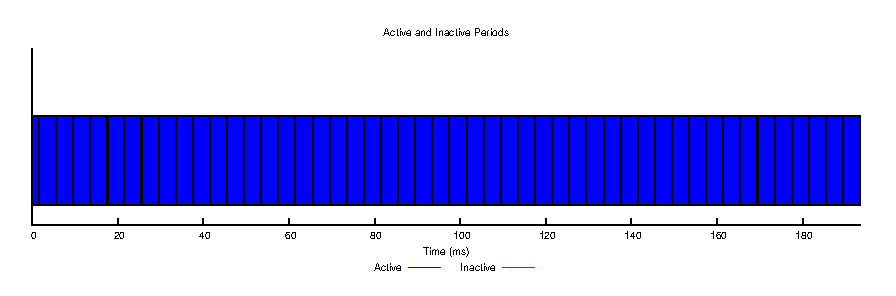
\includegraphics[scale=1]{A1P1.eps}
\end{figure}


\section{Context switches}


% ----------------------------------------------------------------
\end{document}
% ----------------------------------------------------------------
